\documentclass[tikz]{standalone}
\usepackage[utf8]{inputenc}
\usepackage{amsmath}
\usetikzlibrary{intersections}

\begin{document}

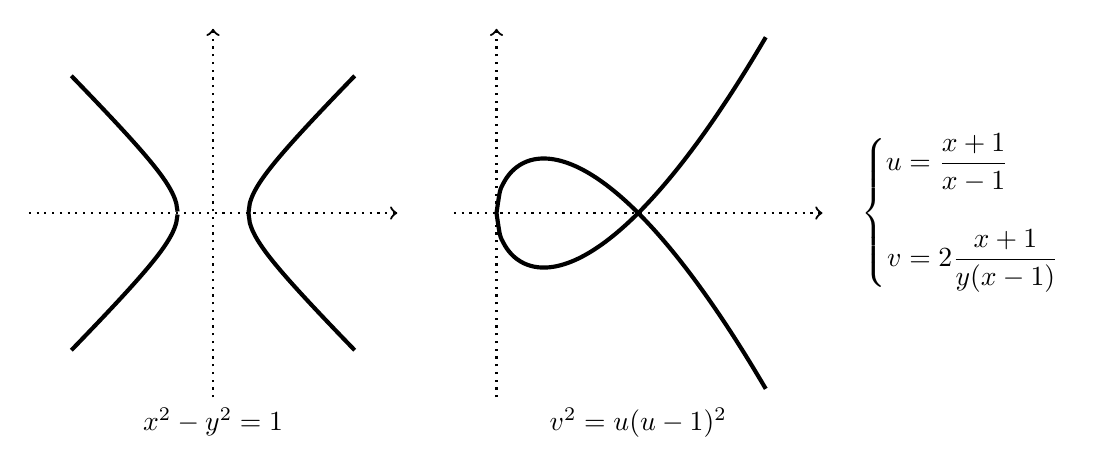
\begin{tikzpicture}[thick,scale=.45]
\def\ptsize{.03}
\draw[->,dotted] (-5.2, 0) -- (5.2,0);
\draw[->,dotted] (0,-5.2) -- (0,5.2);
\path[draw,name path=hyper1,samples=80,line width=1.5pt,domain=-4:-1] plot (\x, {sqrt((\x)^2 - 1)});
\path[draw,name path=hyper2,samples=80,line width=1.5pt,domain=-4:-1] plot (\x, {-sqrt((\x)^2 - 1)});
\path[draw,name path=hyper3,samples=80,line width=1.5pt,domain=1:4] plot (\x, {sqrt((\x)^2 - 1)});
\path[draw,name path=hyper4,samples=80,line width=1.5pt,domain=1:4] plot (\x, {-sqrt((\x)^2 - 1)});
\node[below] at (0,-5.2) {$x^2 - y^2 = 1$};

\begin{scope}[shift={(8,0)},scale=4]
\draw[->,dotted] (-.3, 0) -- (2.3,0);
\draw[->,dotted] (0,-1.3) -- (0,1.3);
\draw[domain=0:1.9,smooth,samples=80,line width=1.5pt] plot (\x, {sqrt(\x)*(\x - 1)});
\draw[domain=0:1.9,smooth,samples=80,line width=1.5pt] plot (\x, {-sqrt(\x)*(\x - 1)});
\node[below] at (1,-1.3) {$v^2 = u(u-1)^2$};
\node[right] at (2.5,0) {\hbox{$\left\{\begin{aligned}u &= \frac{x+1}{x-1} \\[10pt] v&=2\frac{x+1}{y(x-1)}\end{aligned}\right.$}};
\end{scope}

\end{tikzpicture}

\end{document}